% Overleaf: upload this folder (or its ZIP), select main.tex, compiler pdfLaTeX.
% The PDF is compiled from this file. Map and numerical evidence are measured outputs.
\documentclass[10pt,a4paper]{article}
\usepackage[margin=14mm,top=12mm,bottom=12mm]{geometry}
\usepackage[T1]{fontenc}
\usepackage{mathptmx,graphicx,booktabs,amsmath}
\usepackage[hidelinks]{hyperref}
\hypersetup{pdftitle={UDrive: Localization and Mapping in Town02},pdfauthor={Intro2AV project group}}
\pagestyle{empty}
\setlength{\parindent}{0pt}
\setlength{\parskip}{4pt}
\setlength{\tabcolsep}{8pt}
\renewcommand{\arraystretch}{1.07}
\newcommand{\AlignT}{25.0498, -110.2836, -0.2246}
\newcommand{\AlignR}{-0.003539, -0.008079, -0.006158}

% Recomputed against the actual submitted PCD; see map_quality_validation.json.
\newcommand{\FinalGroundP}{4.783}


\begin{document}
{\LARGE\bfseries UDrive: Localization and Mapping in Town02}\par
{\small Intro2AV Project 2 \hfill LiDAR--IMU mapping | Group project}
\vspace{3pt}\hrule\vspace{3pt}

\textbf{Approach and implementation.}
Roof LiDAR supplies metric range and environmental geometry; IMU supplies angular motion and acceleration constraints. We use a Python ROS 2 frontend with robust point-to-plane ICP [1] against a rolling submap, keeping gyro-integrated yaw fixed while estimating roll, pitch and translation. An offline backend jointly refines 200 keyframe poses, velocities, gravity and constant IMU biases using the original IMU and 10 validated LiDAR revisit constraints. Supplied mounting transforms relate sensor and vehicle poses. Original firing times and corrected neighboring poses drive motion compensation. Our work includes ICP, calibration/time handling, revisit validation, sparse robust optimization and export, using NumPy, SciPy and ROS 2 [2--4]. Camera, GNSS, reference poses and teacher geometry are excluded from estimation. All 3,962 scan epochs over 198.05 s are processed (one initializing, 3,961 tracking); no reference-filled poses. ROS nodes use recorded simulation time.

\textbf{Localization evaluation.}
After freezing estimation, all 3,962 vehicle poses were matched to the supplied reference at identical timestamps. For each full trajectory we fit one proper rigid SE(3) alignment, with scale fixed to 1; no segment-wise fit or rescaling. GNSS is a separate verification input only. The previous and final versions use the same measurements:

\begin{center}
\begin{tabular}{lrrr}
\toprule
 & Position ATE RMSE & Position error P95 & 1 s translation RPE RMSE\\
\midrule
Previous refinement & 0.25229 m & 0.38834 m & 0.07929 m\\
Final refinement & \textbf{0.24969 m} & 0.40188 m & 0.07978 m\\
\bottomrule
\end{tabular}
\end{center}
\vspace{-5pt}
{\small Final fixed transform: $\mathbf p_{\rm ref}=R\mathbf p_{\rm map}+\mathbf t$,
$\mathbf t=(\AlignT)$ m;
$R=\exp([\mathbf r]_\times)$, $\mathbf r=(\AlignR)$ rad.}

\begin{center}
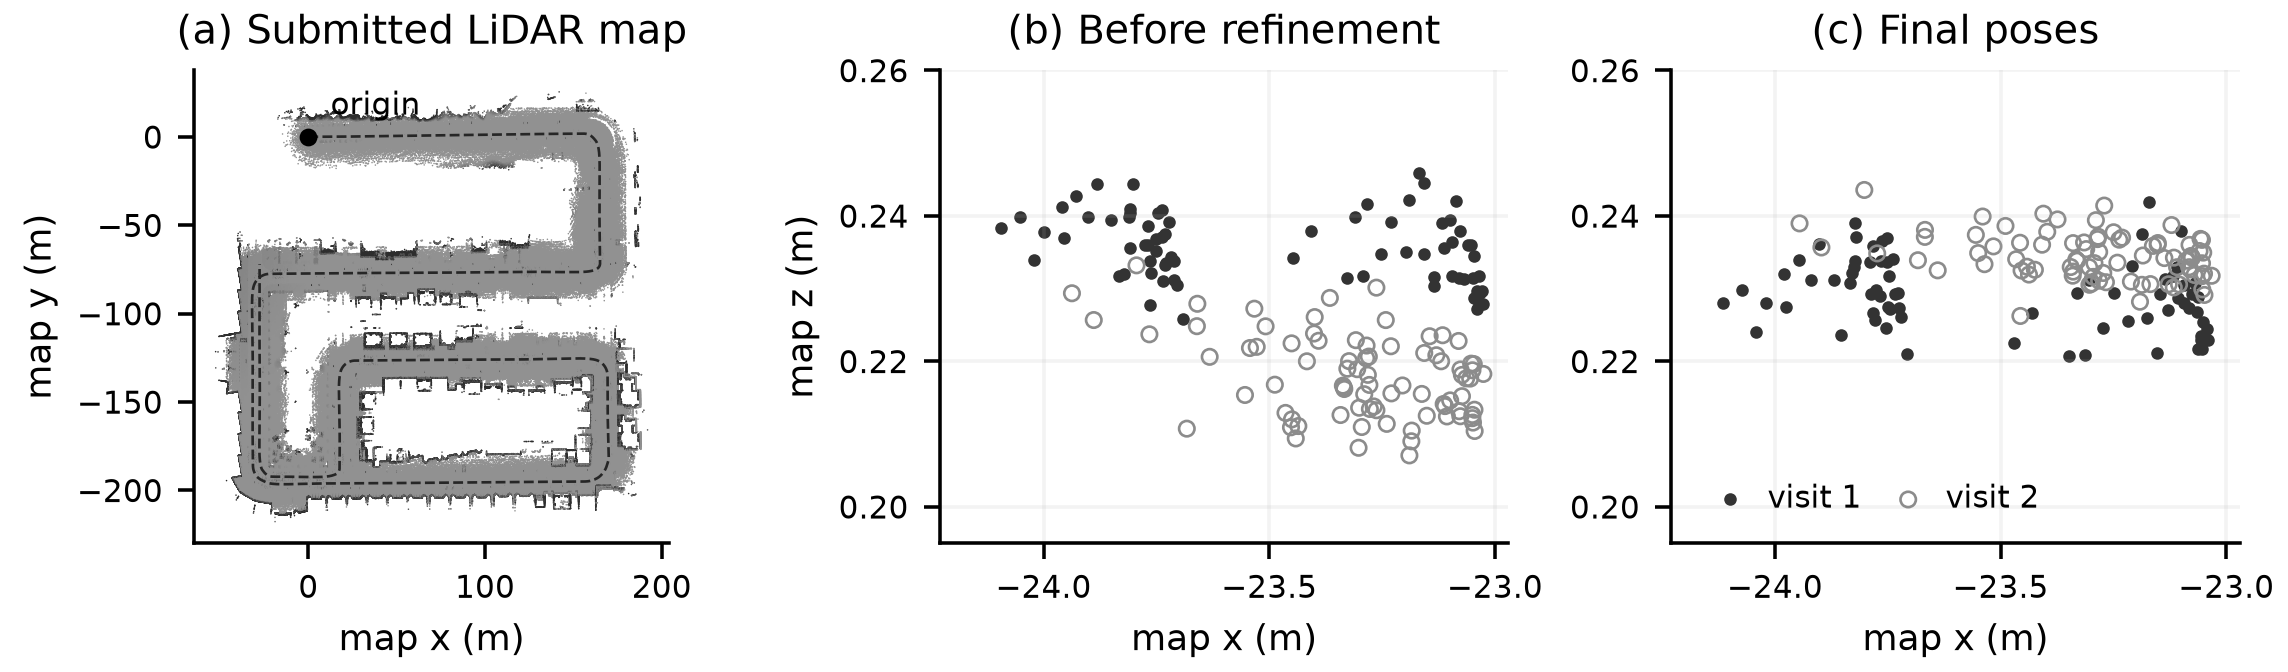
\includegraphics[width=\linewidth]{figures/map_evidence.png}
\end{center}
\vspace{-7pt}
{\small\textbf{Figure 1.} (a) Submitted points, deterministic 1/16 display sample; dashed line: estimated route. (b,c) Same measured returns from two visits, in the same native map axes. The crop is fixed from the previous version; no local alignment, surface fitting or synthetic points.}

\textbf{Map quality.}
At the inspected revisit region, fixed-scan ground/wall point-to-plane residuals decrease from 5.18/6.72 cm to 1.84/4.50 cm. Across 396 scans excluded from map insertion, 396,000 fixed low-surface return IDs have a submitted-map nearest-point distance P95 of \FinalGroundP{} cm. A separate 349,220-return structural cohort has RMSE 19.61 cm (6.83 cm before isolation filtering): removing sparse points worsens tail matches. These are internal consistency checks: the scans still contributed to localization, and the local diagnostic informed configuration selection; they are not independent absolute map accuracy.

\textbf{Engineering problem and limitation.}
Strong attitude priors resisted measured revisit rotations, leaving duplicate surfaces. Increasing revisit rotational weight and relaxing the absolute attitude prior reduced this mismatch; the weights are regularization settings, not calibrated covariances. Overall ATE changes only 2.6 mm and P95 becomes slightly worse. Several dark patches in Fig.~1(a) may reflect local SLAM registration or mapping failures; darkness alone is inconclusive because grayscale also encodes height. Scan-line gaps, residual wall bands and unobserved structures remain. Correlated frontend/IMU factors and mostly planar motion limit gravity/bias separation; this is offline regularized refinement, not fully tightly coupled LIO.

\textbf{Submitted map and viewing.}
\texttt{map.pcd} is binary PCD v0.7, with \textbf{10,272,490 XYZ+RGB points}. Points are retained centroids of measured returns in 0.05 m voxels; a structure-protecting isolation filter removed 1.16\% without moving points. Gray RGB is height-based display color. Coordinates are metres in \texttt{udrive\_map}: origin at the first estimated vehicle pose at scan end; initial vehicle $x$ forward, $y$ left, $z$ up (small initial tilt assumed). Open with \textbf{CloudCompare: File $>$ Open}; no companion map file is required. Coverage is limited to the observed route; neither the input bag nor the teacher map is submitted.

\vspace{2pt}
{\footnotesize\textbf{Sources.}
[1] \href{https://doi.org/10.1109/ROBOT.1991.132043}{Chen \& Medioni, ``Object Modeling by Registration of Multiple Range Images,'' ICRA, 1991}.
[2] \href{https://github.com/ros2/rclpy}{ROS 2 rclpy}.
[3] \href{https://numpy.org/doc/stable/}{NumPy documentation}.
[4] \href{https://docs.scipy.org/doc/scipy/reference/spatial.html}{SciPy spatial} and \href{https://docs.scipy.org/doc/scipy/reference/sparse.linalg.html}{sparse linear algebra}.
}
\end{document}
